\documentclass[a4paper]{article}
\usepackage[utf8]{inputenc}
\usepackage{graphicx}
\usepackage{setspace}
\usepackage{amsmath}
\usepackage{listings}
\usepackage{multirow}
\usepackage{booktabs}
\usepackage[colorlinks,linkcolor=red]{hyperref}
\usepackage{xcolor}
\usepackage[margin=1in]{geometry} 
\usepackage{array} 
\renewcommand\arraystretch{1.4} 
\lstset{
    numbers=left,
    keywordstyle= \color{ blue!70},
    commentstyle= \color{red!50!green!50!blue!50},
    rulesepcolor= \color{ red!20!green!20!blue!20} ,
    escapeinside=``,
    xleftmargin=2em,xrightmargin=2em, aboveskip=1em,
    framexleftmargin=2em,
    language=C++
}
\title{DS $1^{st}$  homework}
\author{58121102 Jiang Yuchu}
\date{September 19 2022}
\begin{document}
\maketitle
\subsubsection*{3. Determine the frequency counts for all statements in the following two program segments:}
\subsubsection*{(a)}
\begin{lstlisting}
for(i=1;i<=n;i++) // n+1 times
  for(j=1;j<=i;j++) // i times for every i -> (1+2+3+4...n)
    for(k=1;k<=j;k++) // j times for every i,j 
      x++;            // -> (1+(1+2)+(1+2+3).....(1+2+3...n))
\end{lstlisting}
Answer:
\begin{table}[htbp]
\centering
\begin{tabular}{cc}
    \toprule
    Line & Frequency Count \\
    \midrule
    1 & n+1 \\
    2 & $\frac{(1+n)n}{2}$ \\
    3 & $\frac{ n(n+1)(n+2)}{6}$ \\
    4 & $\frac{ n(n+1)(n+2)}{6}$ \\
    \bottomrule
    \end{tabular}
\end{table}
\par
\subsubsection*{(b)}
\begin{lstlisting}
i=1; // 1 times
while(i<=n) { // n+1 times
  x++; // n times
  i++; // n times
}
\end{lstlisting}
Answer:
\begin{table}[htbp]
\centering
\begin{tabular}{cc}
    \toprule
    Line & Frequency Count \\
    \midrule
    1 & 1 \\
    2 & n+1 \\
    3 & n \\
    4 & n \\
    \bottomrule
    \end{tabular}
\end{table}
\newpage
\subsubsection*{4. (a) Introduce statements to increment \textit{count} at all appropriate points in Program 1.32.}
\hrule
\begin{lstlisting}
void D(int* x, int n) {
  int i = 1;
  do {
    x[i] += 2;
    i += 2;
  } while(i <= n);
  i = 1;
  while(i <= (n / 2)){
    x[i] += x[i+1];
    i++;
  }
}
\end{lstlisting}
\hrule
\begin{spacing}{1.3}
\noindent \textbf{Program 1.32:} Example Program \par
\noindent Answer:\end{spacing}
\hrule
\begin{lstlisting}
void D(int* x, int n) {
  int i = 1, count = 1;
  do {
    x[i] += 2;
    i += 2;
    count += 3;
  } while(i <= n);
  i = 1, ++count;
  while(i <= (n / 2)){
    x[i] += x[i+1];
    i++;
    count += 3;
  }
  count++;
}
\end{lstlisting}
\hrule

\subsubsection*{(b) Simplify the resulting program by eliminating statements. The simplified program should compute the same value for \textit{count} as computed by the program of (a).}
\begin{spacing}{1.3}
Answer:\end{spacing}
\hrule
\begin{lstlisting}
void D(int* x, int n) {
  int count = 0;
  for (int i = 1; i == 1 || i <= n; i += 2)
    count += 3;
  for (int i = 1; i == 1 || i <= (n / 2); i++)
    count += 3;
  count += 3; // for isolated statements
}
\end{lstlisting}
\hrule
\subsubsection*{(c) What is the exact value of \textit{count} when the program terminates? You may assume that the initial value of \textit{count} is 0.}
\begin{spacing}{1.3}
Answer: \par$count = 3n+3$\end{spacing}
\subsubsection*{(d) Obtain the step count for Program 1.32 using the frequency method. Clearly show the step count table. }
Answer:
\begin{table}[htbp]
\centering
\begin{tabular}{|c|c|c|c|c|c|}
    \hline
    \multirow{2}{*}{Line} & \multirow{2}{*}{S/E} & \multicolumn{2}{c|}{Frequency} & \multicolumn{2}{c|}{Total Steps} \\ \cline{3-6}
                       &                      & n is even           & n is odd          & n is even            & n is odd           \\
    \hline
    2 & 1 & \multicolumn{2}{c|}{1} & \multicolumn{2}{c|}{1} \\
    \hline
    3 & 0 & $\frac{n}{2}$ & $\frac{n+1}{2}$ & \multicolumn{2}{c|}{0}\\
    \hline
    4 & 1 & $\frac{n}{2}$ & $\frac{n+1}{2}$ & $\frac{n}{2}$ & $\frac{n+1}{2}$\\
    \hline
    5 & 1 & $\frac{n}{2}$ & $\frac{n+1}{2}$ & $\frac{n}{2}$ & $\frac{n+1}{2}$\\
    \hline
    6 & 1 & $\frac{n}{2}$ & $\frac{n+1}{2}$ & $\frac{n}{2}$ & $\frac{n+1}{2}$\\
    \hline
    7 & 1 & \multicolumn{2}{c|}{1} & \multicolumn{2}{c|}{1} \\
    \hline
    8 & 1 & $\frac{n}{2} + 1$ & $\frac{n-1}{2} + 1$ & $\frac{n}{2}+1$ & $\frac{n-1}{2}+1$\\
    \hline
    9 & 1 & $\frac{n}{2}$ & $\frac{n-1}{2}$ & $\frac{n}{2}$ & $\frac{n-1}{2}$\\
    \hline
    10 & 1 & $\frac{n}{2}$ & $\frac{n-1}{2}$ & $\frac{n}{2}$ & $\frac{n-1}{2}$\\
    \hline
    11 & 0 & $\frac{n}{2}$ & $\frac{n-1}{2}$ & \multicolumn{2}{c|}{0}\\
    \hline
    \end{tabular}
\end{table}
\newpage
\subsubsection*{10. Obtain the average run time of function BinarySearch (Program 1.10) Do this for suitable values of n in the range [0,100]. Your report must include a plan for the experiment as well as the measured times. These times are to be provided both in a table and as a graph.}
\begin{spacing}{1.3}
Answer:\par
Here is what the BinarySearch looks like:
\end{spacing}
\hrule
\begin{lstlisting}
int BinarySearch(int* a, const int x, const int n) {
    int left = 0, right = n - 1;
    while (left <= right) {
        int middle = (left + right) / 2;
        if (x < a[middle])
            right = middle - 1;
        else if (x > a[middle])
            left = middle + 1;
        else
            return middle;
    }
    return -1;
}
\end{lstlisting}
\hrule
First, search each value from [0, 100] in the range [0, 100]. Second, repeat searching operation for every n for $5\times10^7$ times. Third, calculate the total running time and average running time. Then, ouput the result into data.csv. Finally, draw the graph of the data by python. \href{run:test.cpp}{Here is cpp code} . \href{run:graph.py}{Here is python code.} \href{run:data.csv}{Here is data table}.
\begin{figure}[htbp]
\centering
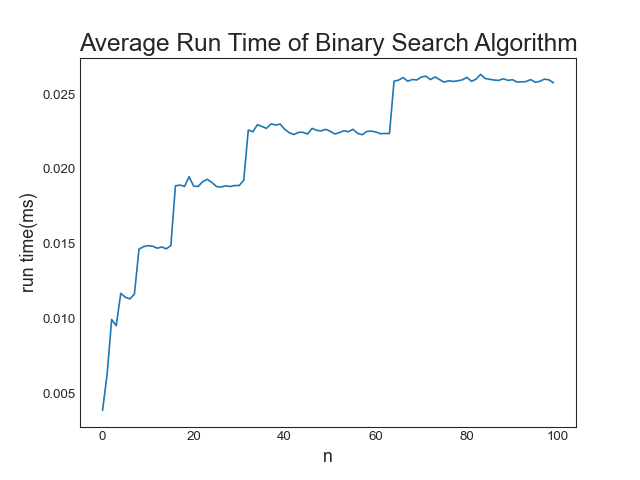
\includegraphics[width=10cm]{Figure_1.png}
\label{2}
\end{figure}
\end{document}
